\documentclass[12pt]{article}
 
\usepackage[margin=1in]{geometry} 
\usepackage{amsmath,amsthm,amssymb,bm}
\usepackage{graphicx}
%\usepackage{subcaption} % To use subfigures with subcaptions
\usepackage[caption = false]{subfig}
 
\begin{document}
  
\title{Task 2. Mesh Animation}
\author{Garoe Dorta-Perez\\
CM50245: Computer Animation and Games II}
 
\maketitle
 
\section{Introduction}

Generating a realistic mesh which is a morphing of two given meshes can be a challenging task.
We present two approaches to produce a intermediate 3D mesh from conforming source and target 3D meshes. 

\section{Linear interpolation}

Linear interpolation is a simple and intuitive first approach.
The new position of a vertex $\mathbf{v}_{it} = \left[ v_{ix}, v_{iy}, v_{iz}\right]^T $ in an interval $t = \lbrace 0, \ldots, 1 \rbrace$ is given by

\begin{equation*}
\mathbf{v}_{it} = (1 - t) \mathbf{p}_i + t \mathbf{q}_i \quad i \in \lbrace 1, \ldots, n \rbrace,
\end{equation*}

where $n$ is the number of vertices, $\mathbf{p}_i = \left[ p_x, p_y, p_z\right]^T$ and $\mathbf{q}_i = \left[ q_x, q_y, q_z\right]^T$ are corresponding vertices in the source and target meshes respectively.
Some meshes generated with this method are shown in Figure \ref{fig:linearInterpolation}.

\section{As rigid as possible interpolation}

The previous method produces distorted meshes due to its non-rigid nature.
One way to produce better results is to use transform-based techniques \cite{Alexa2000}.
Lets define an affine transformation from $\mathbf{p}_i$ to $\mathbf{q}_i$ such that

\begin{align*}
A \mathbf{p}_i + \mathbf{l} = \begin{pmatrix}
 a_{11} & a_{12} & a_{13} \\ 
 a_{21} & a_{22} & a_{23} \\ 
 a_{31} & a_{32}  & a_{33} 
\end{pmatrix} 
\begin{pmatrix}
 p_{ix} \\ 
 p_{iy} \\ 
 p_{iz} 
\end{pmatrix} +
\begin{pmatrix}
 l_x \\ 
 l_y \\ 
 l_z
\end{pmatrix} = \mathbf{q}_i.
\end{align*}

We have a matrix $A_{j}$ and a translation vector $\mathbf{l}_j$ for each triangle, since there are 12 unknowns and each triangle only gives 9 equations, we add an extra point to be able to compute $A_j$.
This new point is computed as $\mathbf{p}_{new} = \mathbf{c}_{tr} + w\mathbf{n}_{tr}$, where $\mathbf{c}_{tr}$ is the triangle centroid, $w$ is the average triangle edge length and $\mathbf{n}_{tr}$ is the triangle normal. 
Mesh vertices are shared among different triangles, so we cannot apply $A_j$ directly.
Instead lets define $B_{j}$ as the matrix that would transform the vertices consistently.
Where $A_j$ and $B_j$ are related by

\begin{equation*}
E(t) = \sum_{j}^J \left \| A_j(t) - B_j(t) \right \|^2_F,
\end{equation*}

where $\left \| \cdot \right \|_F$ is the matrix Frobenius norm, and the objective is to minimize $E(t)$.
If we ignore all the $\mathbf{l}_j$ terms, rename $\mathbf{q}_i$ to treat each vertex in individual vertex in the mesh as $\mathbf{v}_i$ the mesh, and rearrange $B$ such that

\begin{equation*}
PB_{col} = 
\begin{pmatrix}
 \mathbf{p}_1^T & \mathbf{0} & \mathbf{0} \\ 
 \mathbf{0} & \mathbf{p}_1^T & \mathbf{0}\\ 
 \mathbf{0} & \mathbf{0} & \mathbf{p}_1^T \\
  \mathbf{p}_2^T & \mathbf{0} & \mathbf{0} \\ 
 \mathbf{0} & \mathbf{p}_2^T & \mathbf{0}\\ 
 \mathbf{0} & \mathbf{0} & \mathbf{p}_2^T \\
  \mathbf{p}_3^T & \mathbf{0} & \mathbf{0} \\ 
 \mathbf{0} & \mathbf{p}_3^T & \mathbf{0}\\ 
 \mathbf{0} & \mathbf{0} & \mathbf{p}_3^T 
\end{pmatrix}
\begin{pmatrix}
b_{11} \\
b_{12} \\
b_{13} \\
b_{21} \\
b_{22} \\
b_{23} \\
b_{31} \\
b_{32} \\
b_{33}
\end{pmatrix} =
\begin{pmatrix} 
v_{1x} \\
v_{1y} \\
v_{1z} \\
v_{2x} \\
v_{2y} \\
v_{2z} \\
v_{3x} \\
v_{3y} \\
v_{3z}
\end{pmatrix} ~
\text{and} ~
P^{-1} = 
\begin{pmatrix}
\alpha_1 & 0 & 0 & \delta_1 & 0 & 0 & \lambda_1 & 0 & 0 \\
\alpha_2 & 0 & 0 & \delta_2 & 0 & 0 & \lambda_2 & 0 & 0 \\
\alpha_3 & 0 & 0 & \delta_3 & 0 & 0 & \lambda_3 & 0 & 0 \\
0 & \beta_1 & 0 & 0 & \epsilon_1 & 0 & 0 & \mu_1 & 0 \\
0 & \beta_2 & 0 & 0 & \epsilon_2 & 0 & 0 & \mu_2 & 0 \\
0 & \beta_3 & 0 & 0 & \epsilon_3 & 0 & 0 & \mu_3 & 0 \\
0 & 0 & \gamma_1 & 0 & 0 & \kappa_1 & 0 & 0 & \pi_1 \\
0 & 0 & \gamma_2 & 0 & 0 & \kappa_2 & 0 & 0 & \pi_2  \\
0 & 0 & \gamma_3 & 0 & 0 & \kappa_3 & 0 & 0 & \pi_3
\end{pmatrix},
\end{equation*}

then we have that $B = P^{-1}V$.
We would have the above system for each triangle in the mesh, with its own $P$ and $B$ matrices.  
Writing explicitly the Frobenius terms in $E(t)$, and expressing $B$ as a linear combination of $\mathbf{v}_i$, we get

\begin{align*}
E(t) &= \lbrace a_{11}^2 + a_{12}^2 + \ldots + a_{33}^2 + \alpha_1^2 v_{1x}^2 + \ldots + \pi^2 v_{3z}^2 - 2 a_{11} \alpha_1 v_{1x} \\
& - 2 a_{11} \delta_1 v_{2x} - 2 a_{11} \lambda_1 v_{3x} - \ldots - 2 a_{33} \pi_3 v_{3z} + 2 \alpha_1 v_{1x} \delta_1 v_{2x} \\ 
& + 2 \alpha_1 v_{1x} \lambda_1 v_{3x} + \ldots + 2 \kappa_3 v_{2z} \pi_3 v_{3z} \rbrace_{j = 1} + \ldots + \lbrace \cdots \rbrace_{j = J},
\end{align*}

where we have a $\lbrace \cdots \rbrace_j$ term for each triangle.
If we set the transformation of $\mathbf{v_1}$ by linear interpolation, and defining 
$\mathbf{u}(t)^T = \begin{pmatrix} 1, v_{2x}, v_{2y}, v_{2z}, \ldots, v_{mx}, v_{my}, v_{mz} \end{pmatrix}$, where $m$ is the number of vertices, we can stack the terms in a quadratic matrix form 

\begin{equation*}
E(t) = \mathbf{u}^T  \begin{pmatrix}
c & \mathbf{g}(t)^T \\
\mathbf{g}(t) & H
\end{pmatrix} \mathbf{u},
\end{equation*}

where $c$ are the constant coefficients, $\mathbf{g}$ is a vector with the linear terms and $H$ is matrix with the quadratic and mixed terms.
Note that, since $\mathbf{v}_1$ is known, the terms were it appears, become constants or linear in $\mathbf{v}_j$ for $j \neq 1$.
Setting the gradient to zero,

\begin{equation*}
H \mathbf{u}(t) = -\mathbf{g}(t) ~ \rightarrow ~ \mathbf{u}(t) = - H ^{-1} \mathbf{g}(t).
\end{equation*}

Since $H$ is independent on $t$, for each iteration we only need to compute the linear interpolation of $\mathbf{v}_1$ and the new $\mathbf{g}(t)$ to solve the system.

\section{Results and conclusions}

Figure \ref{fig:linearInterpolation} shows that applying a vertex based linear interpolation, rescales the interpolated mesh in unnatural positions.
For example, the horse head and tail shapes in Figure \ref{fig:linearHorse1} are smaller than their counterparts in the source and target shape.
Applying the as-rigid-as-possible interpolation produces better results, because it interpolates the transformation matrices instead of the vertex positions.

\begin{figure}
\subfloat[fig 3]{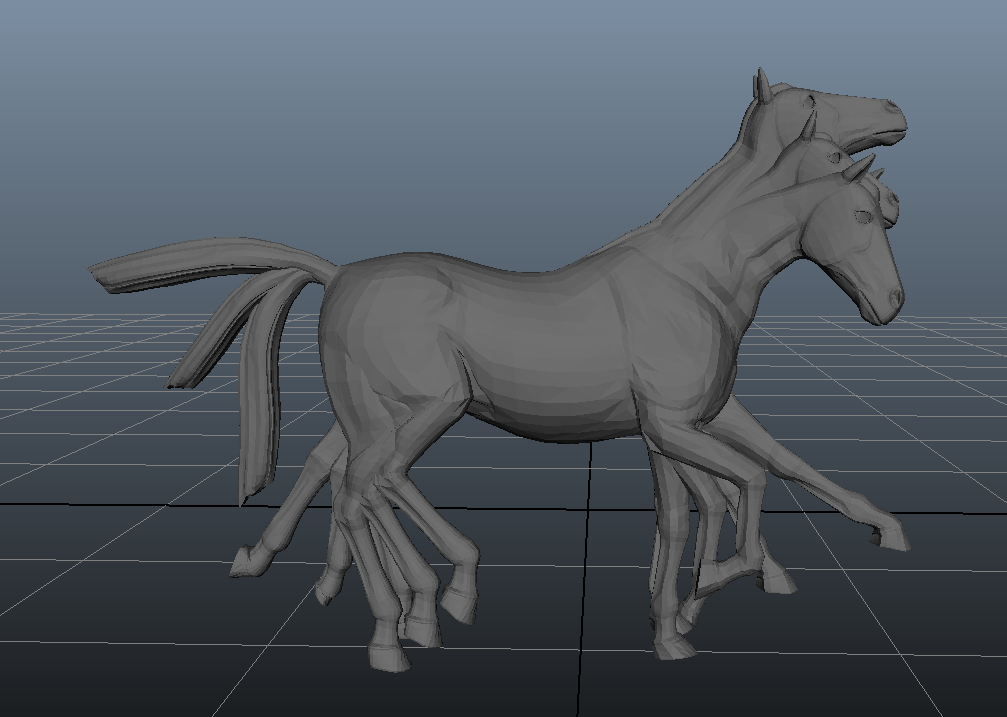
\includegraphics[width = 3in]{images/linearInterpolation1} \label{fig:linearHorse1}}
\subfloat[fig 4]{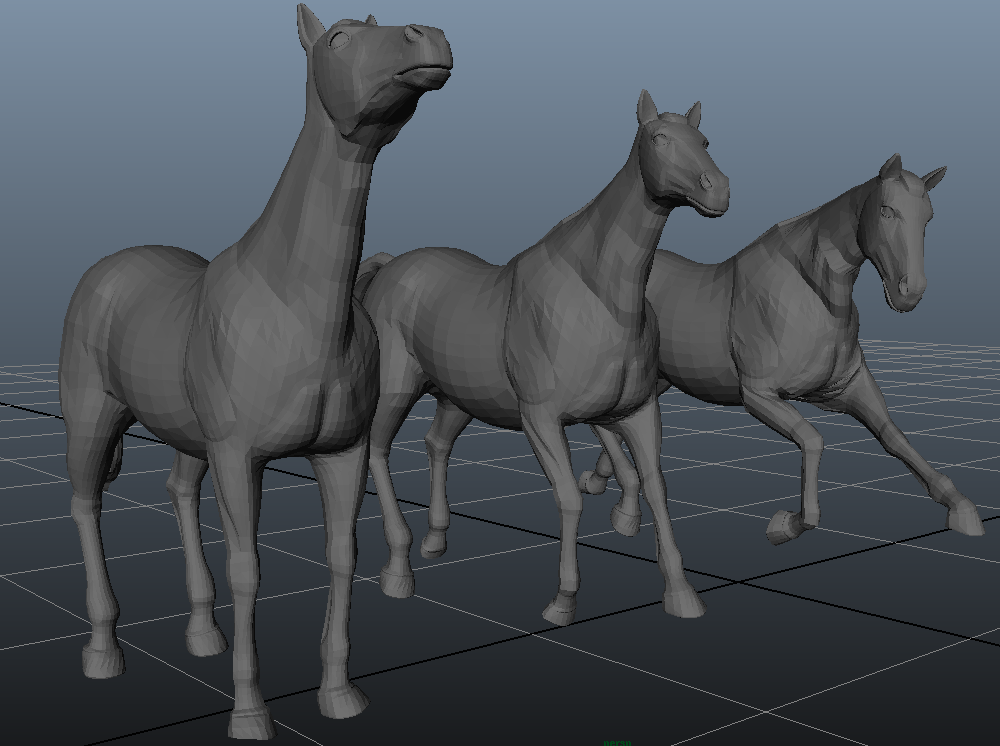
\includegraphics[width = 3in]{images/linearInterpolation2}}\\
\subfloat[fig 1]{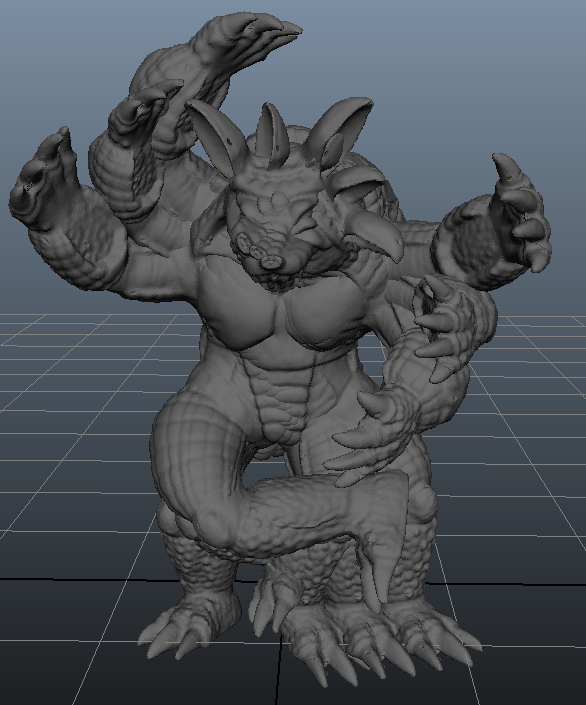
\includegraphics[width = 1.8in]{images/armadillo2}}
\subfloat[fig 2]{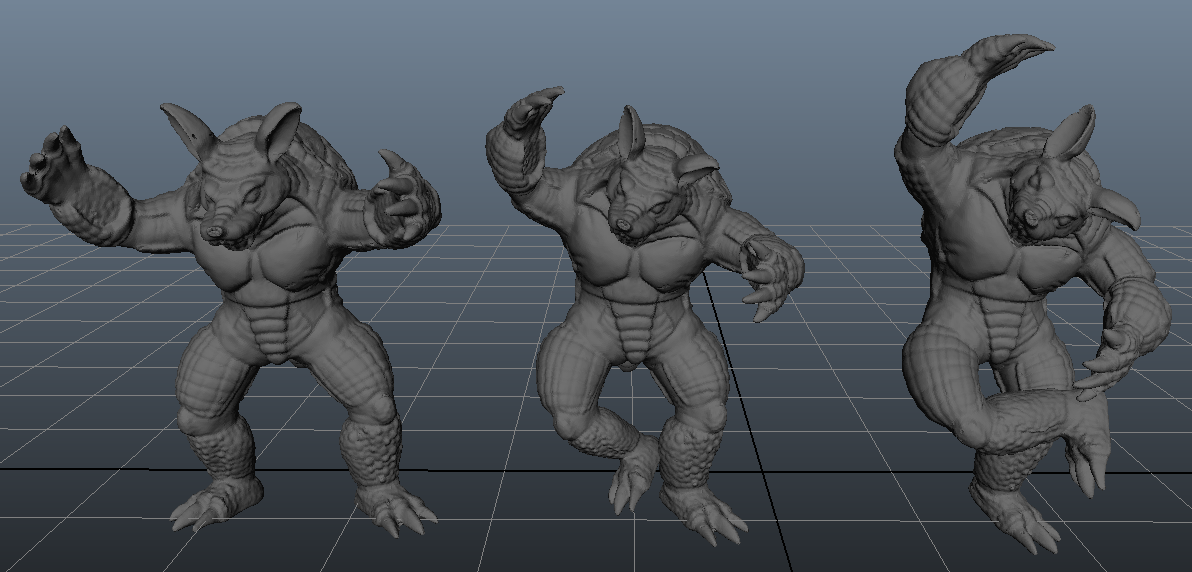
\includegraphics[width = 3.3in]{images/armadillo1}} 
\caption{Horse and armadillo meshes, morphed mesh is in the middle.}
\label{fig:linearInterpolation}
\end{figure}

\bibliographystyle{plain}
\bibliography{t2_meshAnim}

\end{document}

